% -*- coding: utf-8 -*-

\documentclass{beamer}
\mode<presentation>
{
\usetheme{Boadilla}
% \usetheme{Malmoe}

% \usetheme{Warsaw}
% \setbeamercovered{transparent}

% \setbeamertemplate{background canvas}[vertical shading][bottom=white,top=structure.fg!25]
% \usetheme{Warsaw}
% \setbeamertemplate{headline}{}
% \setbeamertemplate{footline}{}
% % \setbeamersize{text margin left=0.5cm}


}

\usepackage[french]{babel}
\usepackage[utf8]{inputenc}

\usepackage{times}
\usepackage[T1]{fontenc}

\usepackage{multimedia}

\title[Analyse de la répartition de CAS et WAP]{Analyse de la répartition des gènes CAS et WAP dans les noyaux de cellules HC11}
% \subtitle{Include Only If Paper Has a Subtitle}

\author{Ga\"etan Lehmann}
\institute[INRA]{INRA, UMR 1198; ENVA; CNRS, FRE 2857, Biologie du D\'eveloppement et  Reproduction, Jouy en Josas, F-78350, France.}
\date[Club chromatine - 18/10/2007]{Club chromatine - 18 octobre 2007}
% \subject{Theoretical Computer Science}

% \pgfdeclareimage[height=0.5cm]{university-logo}{university-logo-filename}
% \logo{\pgfuseimage{university-logo}}

\AtBeginSection[]
{
  \begin{frame}<beamer>
    \frametitle{Plan}
    \tableofcontents[currentsection,currentsubsection]
  \end{frame}
}

\AtBeginSubsection[]
{
  \begin{frame}<beamer>
    \frametitle{Plan}
    \tableofcontents[currentsection,currentsubsection]
  \end{frame}
}

\begin{document}

\frame
{
  \titlepage
}

% \frame
% {
%   \frametitle{Plan}
%   \tableofcontents % [pausesections]
% }
  
\section{Fraction de volume érodé}
  \frame
  {
    \frametitle{Fraction de volume érodé}
  }
  
  
\section{Analyse d'image}
  
    \frame
    {
      \frametitle{Les images}
      \begin{itemize}
        \item Trois canaux (noyaux, CAS et WAP) \\
          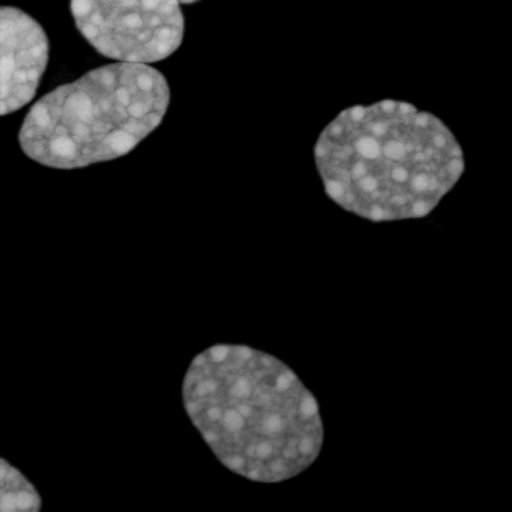
\includegraphics[height=2.5cm]{noyaux.png}
          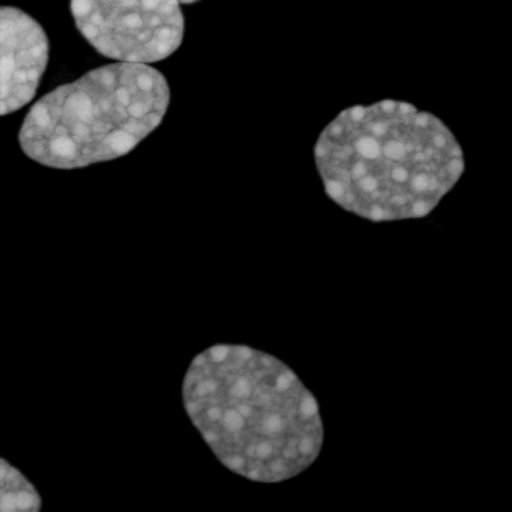
\includegraphics[height=2.5cm]{noyaux.png}
          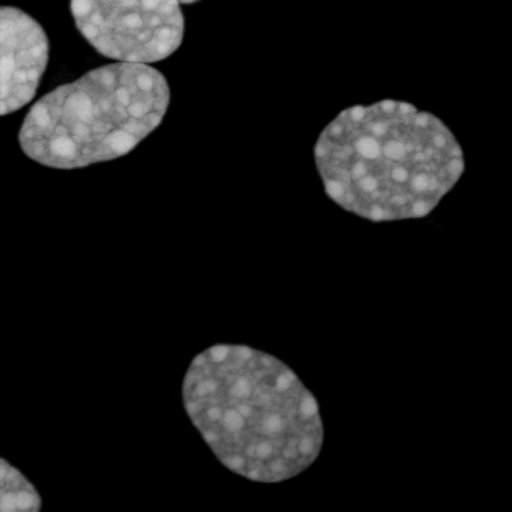
\includegraphics[height=2.5cm]{noyaux.png}
        \item En trois dimensions \\
%           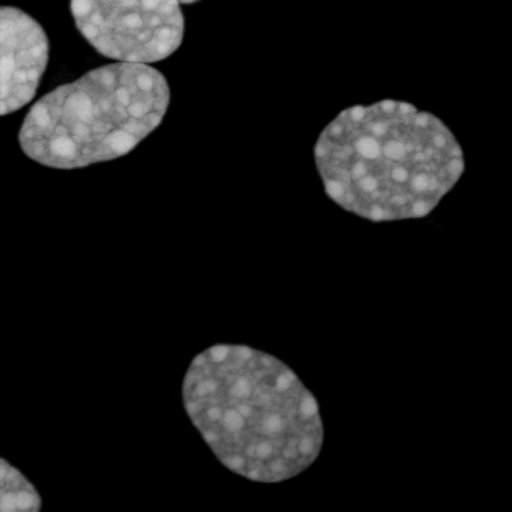
\includegraphics[height=2.5cm]{noyaux.png}
          \movie[width=3.37cm,height=3cm,poster,loop,autostart]{}{vrmaria.avi} % ,externalviewer,showcontrols
      \end{itemize}
    }
    
  \subsection{Débruitage}
    
    \frame
    {
      \frametitle{Débruitage des images de microscopie confocale}
      \begin{itemize}
        \item Filtre médian
        \item Filtre gaussien
      \end{itemize}
    }
    
%     \frame
%     {
%       \frametitle{Débruitage des images de noyaux}
%     }
%     
%     \frame
%     {
%       \frametitle{Débruitage des images de CAS}
%     }
%     
%     \frame
%     {
%       \frametitle{Débruitage des images de WAP}
%     }
    
  \subsection{Segmentation des noyaux}
    
    \frame
    {
      \frametitle{Seuillage, histogramme unimodale et gradient}
      \begin{center}
        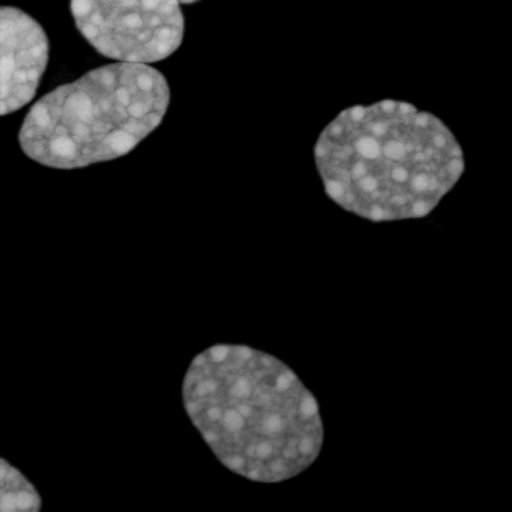
\includegraphics[height=3.8cm]{noyaux.png} %
        \uncover<2->{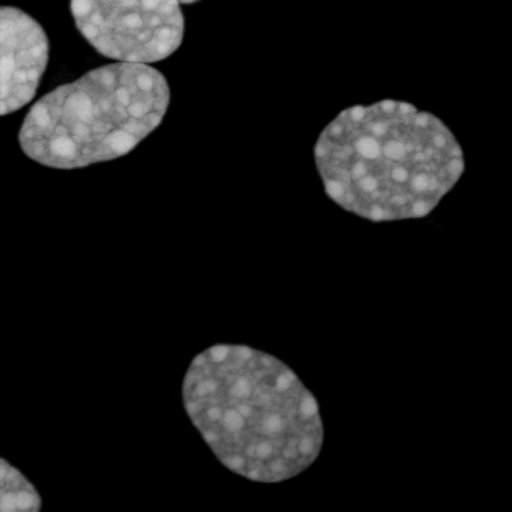
\includegraphics[height=3.8cm]{noyaux.png}}\\ %histogram.png}
        \uncover<3->{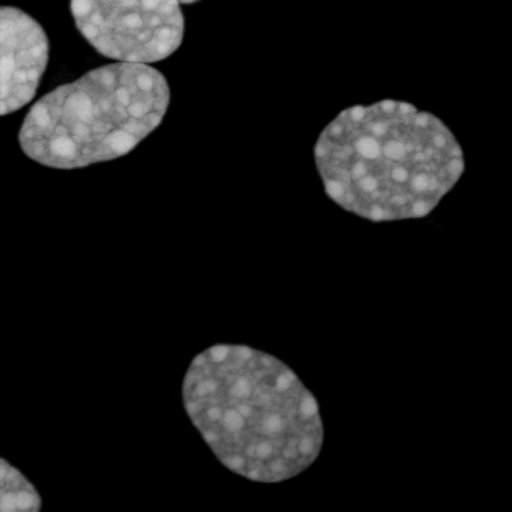
\includegraphics[height=3.8cm]{noyaux.png}} %gradient.png} %
        \uncover<4->{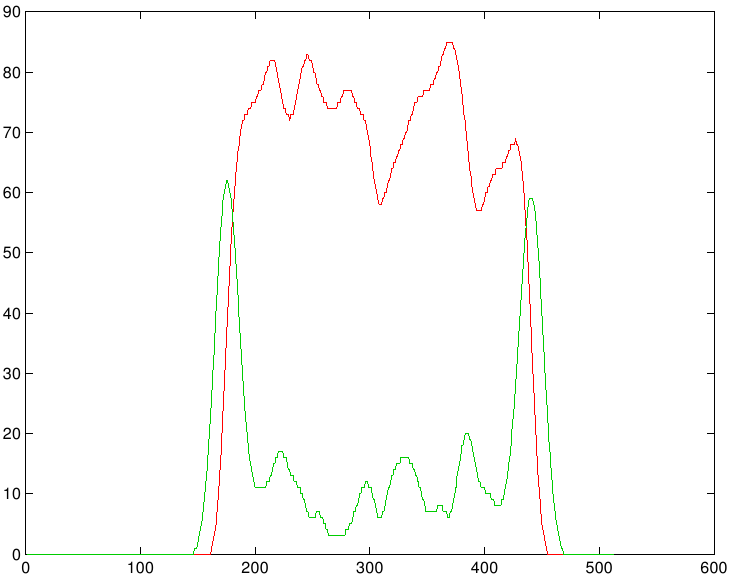
\includegraphics[width=3.8cm]{profile-gradient.png}} %
       \end{center}
   }

    \frame
    {
      \frametitle{Robust Automatic Threshold Selection}
      \begin{itemize}
        \item<1->{Calcul la moyenne des intensités de l'image pondérée par le gradient de l'image.}
        $$
        T = \frac{\sum\limits_{p~in~D}G(p)\only<2->{\alert<2>{^m}}~.~I(p)}{\sum\limits_{p~in~D}G(p)\only<2->{\alert<2>{^m}}}
        $$
        \item<2->{Utilisation d'une puissance du gradient pour diminuer la sensibilité au bruit (en général, $m = 2$).}
        \item<3->{Suppression des petites zones qui perturbent le calcul :}
          \begin{itemize}
            \item avec une ouverture par attribut pour les zone claires,
            \item avec un {\em fill hole} pour les zone sombres.
          \end{itemize}
    
      \end{itemize}
    }
  
    \frame
    {
      \frametitle{Amélioration du masque et labellisation}
    }
    
  
  \subsection{Segmentation des spots de CAS}
    
    \frame
    {
      \frametitle{Tophat par attribut}
      \begin{itemize}
        \item Bon contraste entre le fond et les spots.
        \item Fond de niveau parfois élevé et texturé.
      \end{itemize}
    }
    
    \frame
    {
      \frametitle{Seuillage et labellisation}
    }
    
  \subsection{Segmentation des spots de WAP}
    
    \frame
    {
      \frametitle{Représentation en arbre de composantes}
    }
  
    \frame
    {
      \frametitle{Garder les quatres pics les plus importants}
    }
  
\section{Mesures}
    
  \subsection{Position des gènes}
    
    \frame
    {
      \frametitle{}
    }
    
  \subsection{Fraction de volume érodé}
    
    \frame
    {
      \frametitle{}
    }
    
  \subsection{Distance à la membrane}
    
    \frame
    {
      \frametitle{}
    }
    
  \subsection{Applatissement}
    
    \frame
    {
      \frametitle{}
    }
    
\section{Analyse statistique}
  
  \frame
  {
    \frametitle{}
  }
  
  
\section*{Conclusion}
  
  \frame
  {
    \frametitle{Intéraction entre personnes}
  }
  
\end{document}
